
% ==================================================
%	Theorie
% ==================================================

\section{Theorie}
\label{sec:theorie}

Im Folgenden soll skizzenhaft die Herleitung der benötigten Formeln gezeigt
werden.
Die Probe ist ein 3 bis \SI{5}{\mm} dicker Kristall und dient in einem
Plattenkondensator als Dielektrikum. Das Anlegen einer Spannung führt
schließlich zur einer Ausrichtung der Dipole in Feldrichtung.
Aufgrund der thermischen Bewegung der Gitteratome wird die Ausrichtung
allerdings gestört. Im Mittel wird nur ein Bruchteil $y$ der Dipole
in Feldrichtung zeigen. Für diesen Bruchteil gilt mit der sogenannten
\emph{Langevin}-Funktion
%
\begin{equation}
	y = L(x) = \coth(x) - \frac{1}{x} ~, \quad x \coloneqq \frac{pE}{\kB T} ~,
	\label{eq:langevin}
\end{equation}
%
wobei $E$ die elektrische Feldstärke und $p$ der Betrag des Dipolmomentes ist.
In dem Versuch gilt der Limes $pE \ll \kB T$, sodass für den Bruchteil $y$ nun
%
\begin{equation}
	y(T) = \frac{pE}{3\kB T}
	\label{eq:bruchteil_limes}
\end{equation}
%
gilt.
Nun muss das elektrische Feld eine Zeit, die groß gegen die Relaxationszeit
$\tau(T)$ ist, eingeschaltet sein, damit sich der Bruchteil $y$
ausrichten kann. Anschließend wird der Kristall schnell abgekühlt bis auf
ca. \SI{-40}{\celsius}, sodass der Dipolzustand praktisch eingefroren wird.
Nach den Abkühlen wird der Kondensator für ca. \SI{2}{min}
kurzgeschlossen, um die restlichen beweglichen Elektronen abzuführen.
Zudem wird das elektrische Feld abgeschaltet.
Nun wird die Probe mit einer möglichst konstanten Heizrate
%
\begin{equation}
	b \coloneqq \dv{T}{t} = \text{const}
	\label{eq:heizrate}
\end{equation}
%
erwärmt. Durch die Erwärmung lösen sich die Dipole zunehmend aus ihrer
"`eingefrorenen"' Vorzugsrichtung und nehmen wieder eine statistische
Verteilung an. Dies wird als \emph{Dipolrelaxation} bezeichnet.
Die Dipolrelaxation führt schließlich auf einen Dipolstrom, welcher schließlich
messbar ist. Für die Dipolstromdichte gilt
%
\begin{equation}
	j(T) = y(T_p) \, p \, \dv{N}{t} ~.
	\label{eq:dipolstromdichte}
\end{equation}
%
Hier bezeichnet $T_p$ die Polarisationstemperatur und $N$ die Anzahl der
relaxierten Dipole pro Volumeneinheit. Die Änderung $\dv*{N}{t}$ ist dabei
proportional zur Teilchendichte $N$ der noch orientierten Dipole
zum Zeitpunkt $t$ selbst, sodass hierfür die
Differenzialgleichung
%
\begin{equation}
	\dv{N}{t} = - \frac{N}{\tau(T)}
	\label{eq:dgl}
\end{equation}
%
aufgestellt werden kann. Die Lösung dieser DGL unter Berücksichtigung
von \eqref{eq:heizrate} und \eqref{eq:relaxationszeit} und einsetzen in
\eqref{eq:dipolstromdichte} liefert für die Stromdichte
%
\begin{equation}
	j(T) = \frac{p^2 E}{3\kB T} \frac{N_p}{\tau_0}
		\exp[-\frac{1}{b\tau_0} \int_{T_0}^{T} \exp(-\frac{W}{\kB T'}) \dd{T'}]
		\exp[-\frac{W}{\kB T}] ~. \label{eq:Stromdichte}
\end{equation}
%
Der Verlauf der Stromdichte ist in Abbildung \ref{fig:verlauf} dargestellt.
Da die Kurve am Anfang sehr flach ist, gilt
%
\begin{equation}
	\int_{T_0}^{T} \exp[-\frac{W}{\kB T}] \dd{T'} \approx 0 ~,
\end{equation}
%
womit die Dipolstromdichte zu
%
\begin{equation}
	\boxed{
		j(T) = \frac{p^2 E}{3\kB T} \frac{N_p}{\tau_0} \exp[-\frac{W}{\kB T}] ~.
	}
	\label{eq:dipolstromdichte_1}
\end{equation}
%
genähert werden kann. Diese Form kann zur Bestimmung der Aktivierungsenergie
verwandt werden.
%
\begin{figure}[htpb]
	\centering
	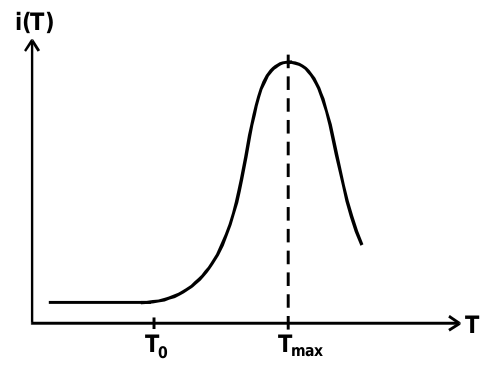
\includegraphics[scale=0.4]{bilder/verlauf.png}
	\caption{Verlauf der Dipolstromdichte. \cite{AP}}
	\label{fig:verlauf}
\end{figure}
%
Desweiteren kann der gesamte Kurvenverlauf zur Bestimmung der
Aktivierungsenergie verwandt werden. Hierzu wird die Polarisation $P$,
welche gleich dem Gesamtdipolmoment pro Volumeneinheit der Probe ist,
betrachtet. Für $P$ gilt eine ähnliche DGL wie \ref{eq:dgl} entsprechend
%
\begin{equation}
	\dv{P}{t} = - \frac{P(t)}{\tau(T(t))} ~.
	\label{eq:dgl_polarisation}
\end{equation}
%
Für den Polarisationsstrom und dessen Integral gilt mit den Probenquerschnitt
$F$
%
\begin{equation}
	i(t) = F \dv{P}{t} ~, \quad \int_{t}^{\infty} i(t) \dd{t} = F P(t) ~.
	\label{eq:pol_strom_und_integral}
\end{equation}
%
Mit \eqref{eq:dgl_polarisation}, \eqref{eq:pol_strom_und_integral},
\eqref{eq:relaxationszeit} und \eqref{eq:heizrate} folgt nun
%
\begin{equation}
	\boxed{
		\frac{W}{\kB T} =
			\frac{1}{\tau_0\, b\, i(T)}\int_{T/b}^{\infty} i(T') \dd{T'} ~.
	}
	\label{eq:Dipolstromdichte_2}
\end{equation}
%
Hiermit kann nun die Aktivierungsenergie durch Auftragen von
%
\begin{equation}
	\frac{1}{\text{const}\cdot i(T)}\int_{T/b}^{T^*} i(T') \dd{T'}
\end{equation}
%
gegen $1/T$ bestimmt werden, wobei $T^*$ so gewählt muss, dass
$i(T^*) \approx 0$ gilt.
